\scanpage{11}
\mspage{10}

I just checked with Siebenmann and a Teichmuller space expert named \unsure{Haritz} -- The situation is this:

\textcircled{1} It is unknown whether every finite subgroup $\Gamma\subseteq$ Teich. group operates on an algebraic curve. But

\textcircled{2} It is true for $\Gamma=$ finite soluble gp +

\textcircled{3} True \deleted{\unsure{also}} for genus $=2$.

\figure{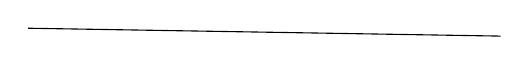
\begin{tikzpicture}\draw (0,0)--(6,-.1);\end{tikzpicture}}

Concerning the hypersurface $Y\subseteq X$ and finite autom. $u$ of $X$ which is \uline{identity} on $\unsure{X|Y}$ -- Siebenmann says that this is certainly solvable using \uline{Smith Theory} (i.e. $u=1$).
